\documentclass{article}

\usepackage[letterpaper, portrait, margin=1.5in]{geometry}

\usepackage{fancyhdr}
\usepackage{ragged2e}
\usepackage{graphicx}
\usepackage{caption}
\usepackage{amsmath}
\usepackage{rotating}

\usepackage{listings}
\usepackage{color}

\definecolor{dkgreen}{rgb}{0,0.6,0}
\definecolor{gray}{rgb}{0.5,0.5,0.5}
\definecolor{mauve}{rgb}{0.58,0,0.82}

\lstset{frame=tb,
  language=Java,
  aboveskip=3mm,
  belowskip=3mm,
  showstringspaces=false,
  columns=flexible,
  basicstyle={\small\ttfamily},
  numbers=none,
  numberstyle=\tiny\color{gray},
  keywordstyle=\color{blue},
  commentstyle=\color{dkgreen},
  stringstyle=\color{mauve},
  breaklines=true,
  breakatwhitespace=true,
  tabsize=4
}

\setcounter{secnumdepth}{1}

\usepackage{chngcntr}
\counterwithin{figure}{section}

\renewcommand*{\thepage}{C\arabic{page}}

\pagestyle{fancy}
\lhead{ACME Robotics}
\chead{\#8367}
\rhead{\ifcontents Contents \else Week \thesection \fi}

\newif\ifcontents
\contentstrue

\makeatletter
\renewcommand{\@seccntformat}[1]{}
\makeatother
\begin{document}

\subsection{Attaching New Lift}
After the completion of the lift, Oren was able to easily bolt the lift to the robot, wire it and temporarily check it under load and observe it running during a match. It was quickly noticed that near the top end of the lift's throw, there was to much deviation of the outside rails. Causing the lift to bind and fall off the bearing runners (Picture), to fix this the cross plate holding the two outside rails would need to be remade, so that it would pull the rails closer together to ensure both were perpendicular to the drive train. 

\subsection{New cross plate}
  A new cross plate needed to be made because the one ACME took to NorCals was made in the room and had many extraneous holes. The new lift was also being mounted at the same time and the cross plate needed to be refitted to reduce slop and increase the strength of the subsystem. The old plate was also ugly and made the over all design look very unprofessional. To improve this a new plate was manufactured with the team name engraved and mounting holes pre-drilled for accuracy. This improved the structural integrity of the lift and added to the custom look of the robot.
  
  \begin{figure}
    \centering
    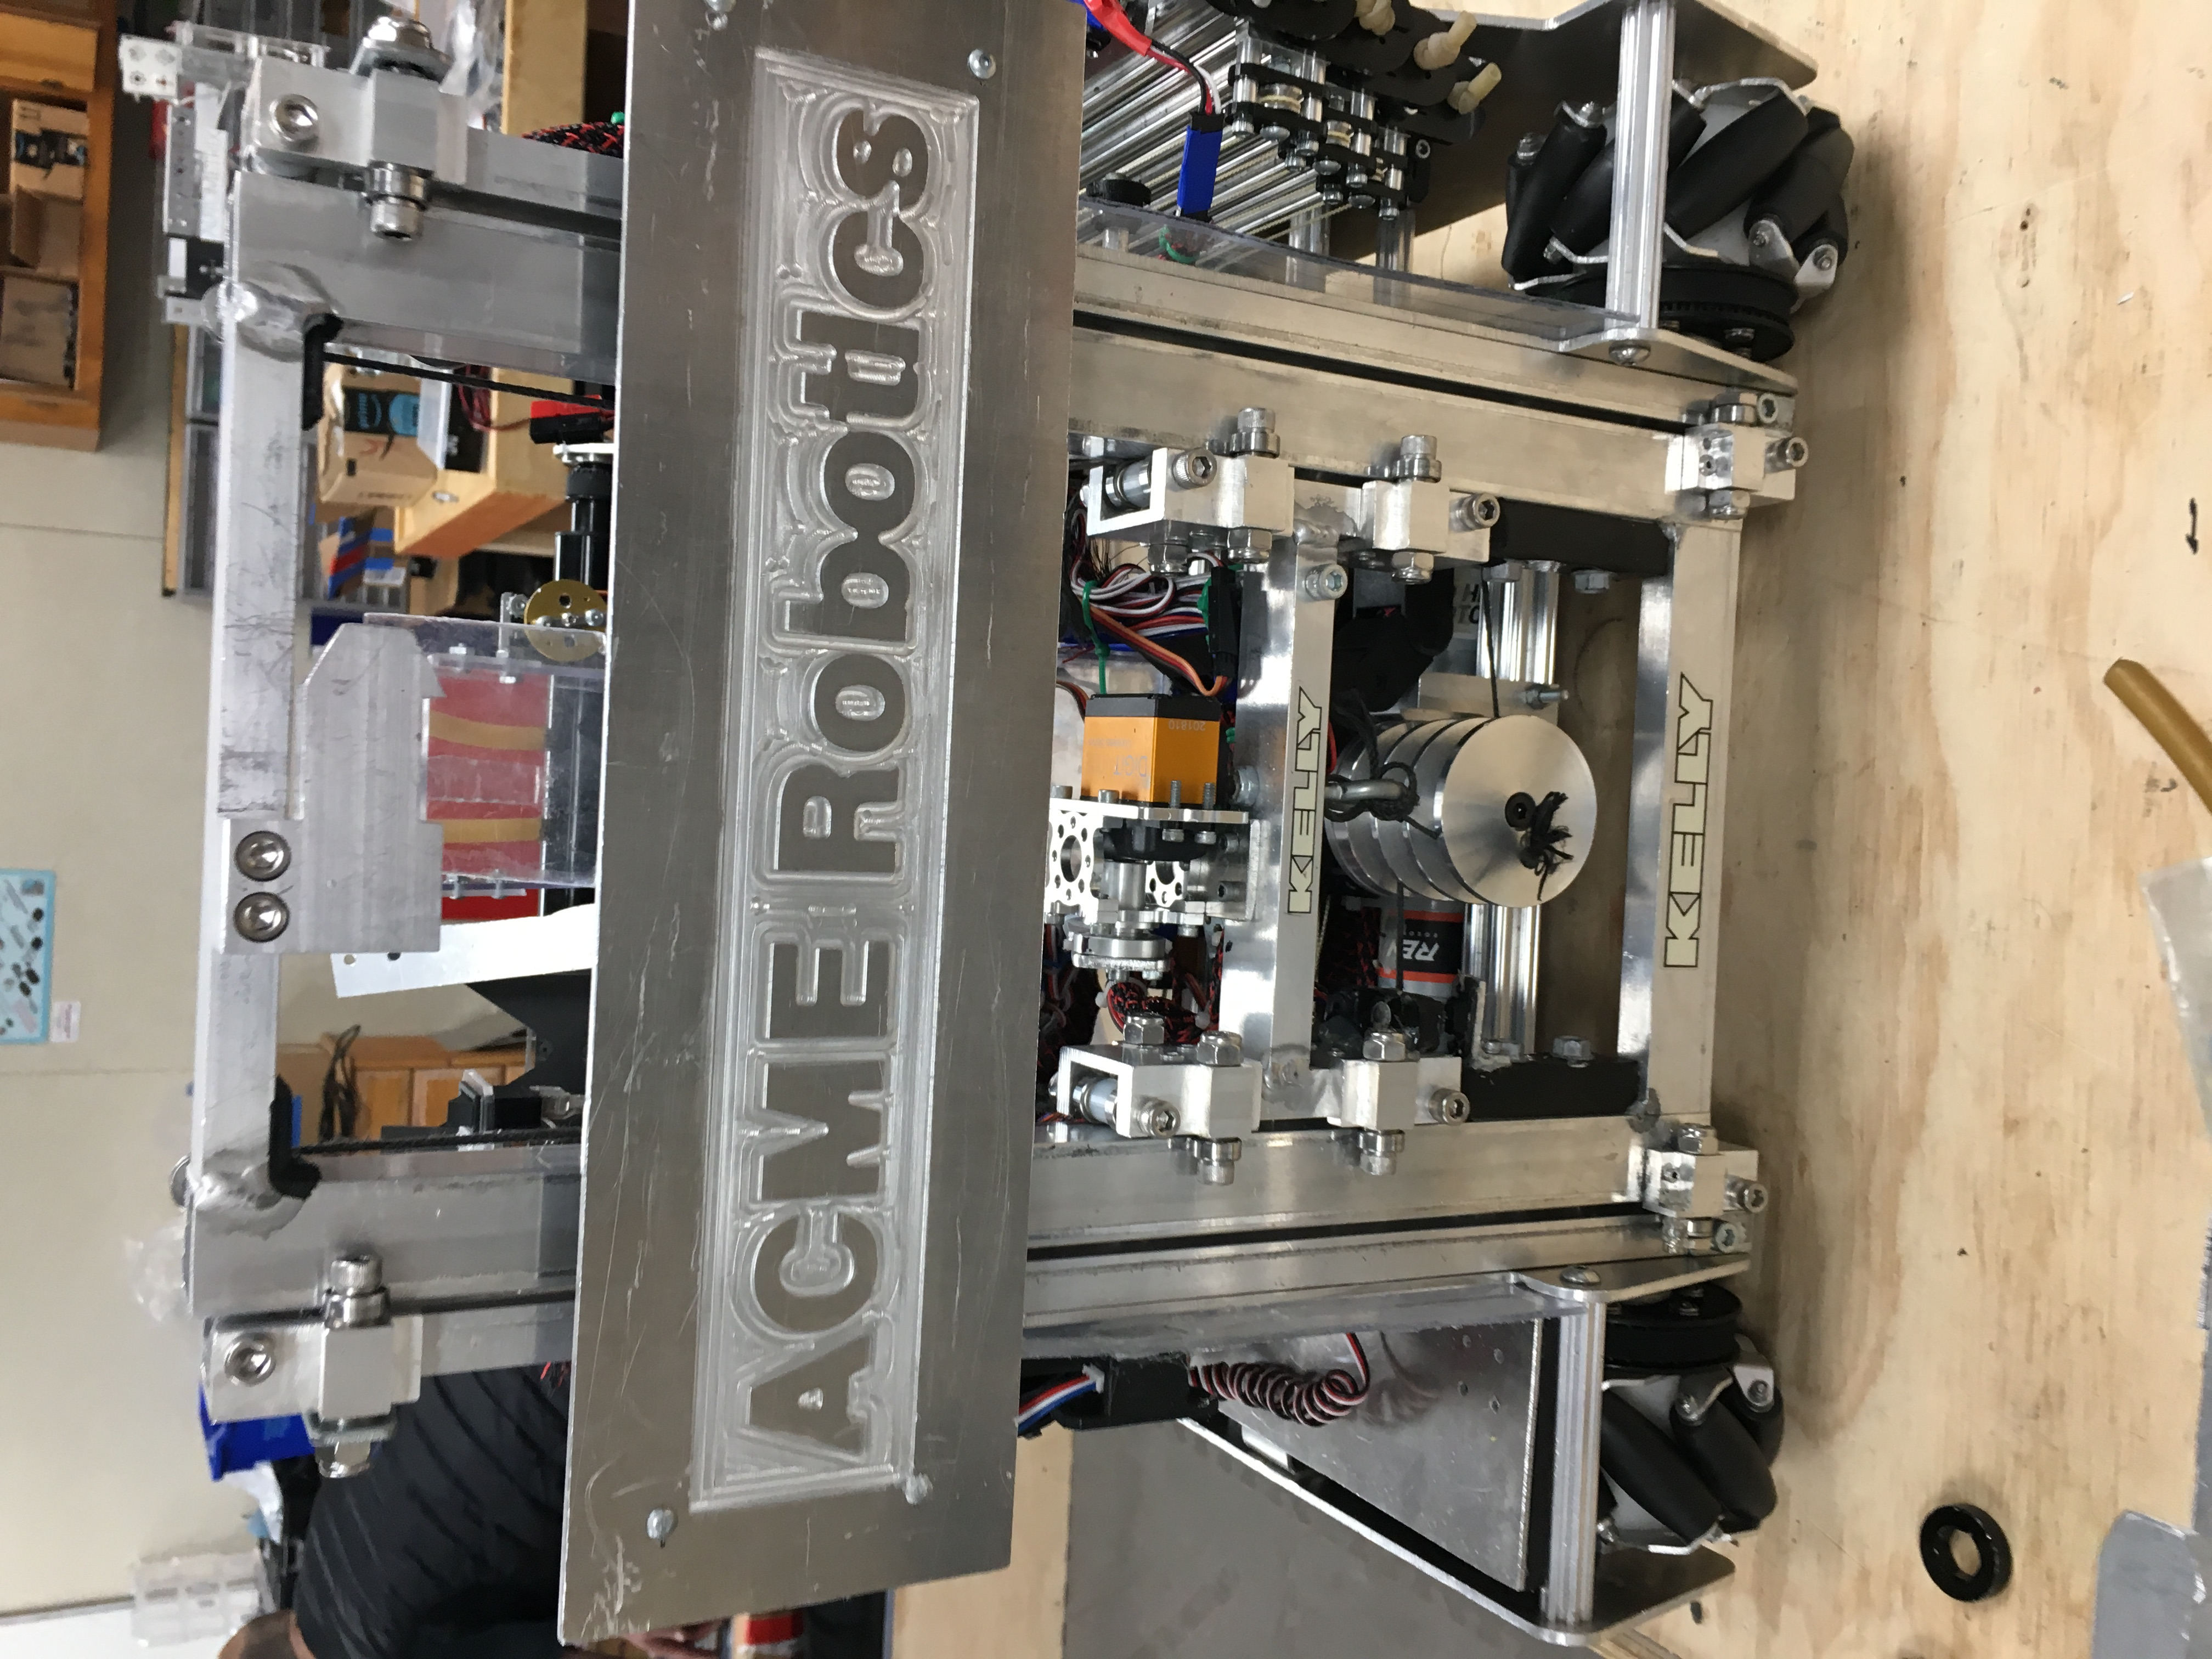
\includegraphics[width= 0.5 \textwidth, angle=270]{28_03-11/images/crossplate.JPG}
    \caption{Finished Cross Plate on the Robot}
    \label{fig:plate}
\end{figure}

 
\end{document}